\textbf{Softwarové inženýrství} je inženýrská disciplína zabývající se praktickými problémy vývoje
rozsáhlých softwarových systémů.

\subsection{Softwarový proces}
\textbf{Softwarový proces} je po částech uspořádaná množina kroků směřujících k vytvoření nebo úpravě softwarového díla.
\begin{itemize}
\item Krokem může být \textbf{aktivita} nebo opět \textbf{podproces} (hierarchická dekompozice procesu). 
\item Aktivity a podprocesy mohou \textbf{probíhat v čase souběžně}, tudíž je vyžadována jejich koordinace. 
\item Je \textbf{nutné zajistit opakovatelnost použití procesu ve vztahu k jednotlivým softwarovým projektům}, tedy zajistit jeho \textbf{znovupoužitelnost}.  Cílem je dosáhnout stabilních výsledků vysoké úrovně kvality.
\item Řada činností je zajišťována lidmi vybavenými určitými schopnostmi a znalostmi a majícím k dispozici technické prostředky nutné pro realizaci těchto činností.
\item \textbf{Softwarový produkt} je realizován v kontextu organizace s danými ekonomickými možnostmi a organizační strukturou.
\end{itemize}

\subsection{Vyspělost úrovně}
Úroveň definice a využití softwarového procesu je hodnocena dle stupnice \textbf{SEI (Software Engineering Institute)} \textbf{1 - 5} vyjadřující vyspělost firmy či organizace z daného hlediska. Tento model hodnocení vyspělosti a schopností dodavatele softwarového produktu se nazývá \textbf{CMM (Capability Maturity Model)} a jeho jednotlivé úrovně lze stručně charakterizovat asi takto:

\begin{enumerate}
\item \textbf{Počáteční (Initial)} - firma \textbf{nemá definován softwarový proces} a každý projekt je řešen \textbf{případ od případu} (ad hoc).
\item \textbf{Opakovatelná (Repeatable)} - firma identifikovala v jednotlivých projektech \textbf{opakovatelné postupy} a tyto je schopna reprodukovat v každém novém projektu.
\item \textbf{Definovaná (Defined)} - softwarový proces je \textbf{definován (a dokumentován)} na základě integrace dříve identifikovaných opakovatelných kroků.
\item \textbf{Řízená (Managed)} - na základě definovaného softwarového procesu je firma schopna jeho \textbf{řízení} a \textbf{monitorování}.
\item \textbf{Optimalizovaná (Optimized)} - zpětnovazební informace získaná \textbf{dlouhodobým procesem monitorování} softwarového procesu je využita ve prospěch jeho optimalizace.
\end{enumerate}

\subsection*{Modely softwarového procesu}
\subsection{Vodopádový model}
Základem téměř všech modelů softwarového procesu se stal vodopádový model. Tento vodopádový model vychází z \textbf{rozdělení životního cyklu softwarového díla} na čtyři základní fáze:
\begin{enumerate}
\item Analýza požadavků a jejich specifikace.
\item Návrh softwarového systému.
\item Implementace.
\item Testování a udržování vytvořeného produktu.
\end{enumerate}
Princip vodopádu spočívá v tom, že \textbf{následující množina činností spjatá s danou fází} nemůže započít dříve, než skončí předchozí. Jinými slovy řečeno, výsledky předchozí fáze „vtékají“ jako vstupy do fáze následující.
\\\\
\noindent\makebox[\textwidth]{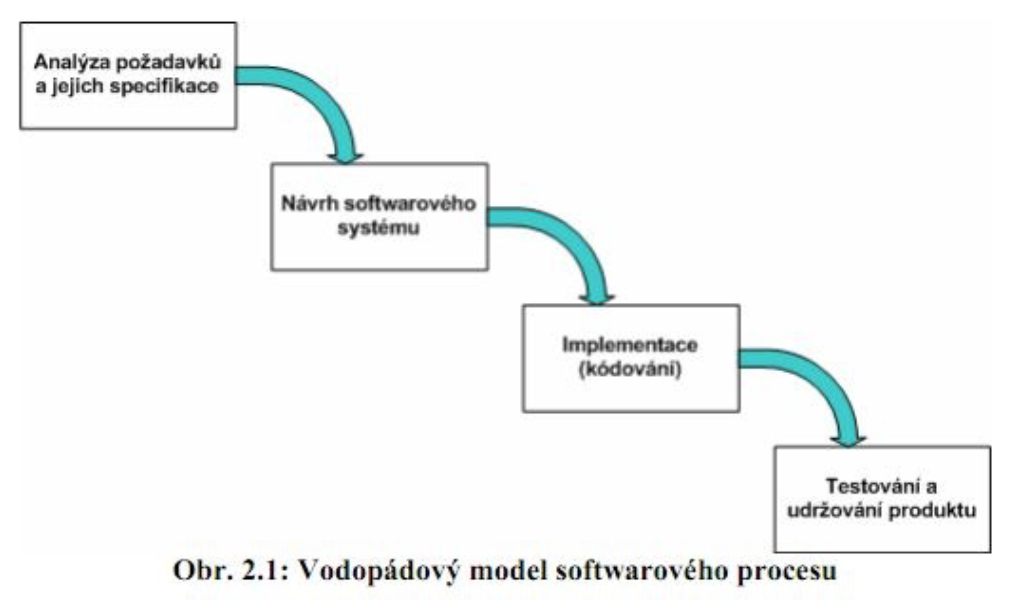
\includegraphics[width=12cm]{assets/swi1}}
Model je možno v \textbf{různých modifikacích} a \textbf{rozšířeních} nalézt ve většině současných přístupů. Tyto modifikace vznikly především kvůli odstranění některých jeho \textbf{nedostatků}, mezi které patří:
\begin{itemize}
\item \textbf{Prodleva} mezi zadáním projektu a vytvořením spustitelného systému je příliš dlouhá.
\item \textbf{Výsledek závisí} na \textbf{úplném a korektním zadaní požadavků} kladených na výsledný produkt.
\item \textbf{Nelze odhalit výslednou kvalitu produktu} danou splněním všech požadavků, dokud není výsledný softwarový systém hotov.
\end{itemize}

\subsubsection{Modifikace Vodopádového modelu}
\begin{itemize}
\item \textbf{Inkrementální}: \textbf{postupné vytváření verzí} softwaru zahrnujících postupně širší spektrum funkcí definovaných postupně v průběhu jeho vytváření. V podstatě se jedná o více menších vodopádů provedených za sebou tak, aby každý z nich odpovídal nové sadě doplněných požadavků.
\item \textbf{Spirálový}: zahrnuje do svého \textbf{životního cyklu další fáze} jako je vytvoření a hodnocení \textbf{prototypu} ověřující funkcionalitu cílového systému, přičemž \textbf{každý cyklus nabaluje další požadavky} specifikované zadavatelem.
\end{itemize}


\subsection{RUP (Rational Unified Process)}
Rational Unified Process (RUP) je \textbf{metodika vývoje softwaru} vytvořená společností Rational Software Corporation. Je použitelná pro \textbf{jakýkoliv rozsah projektu}, ale díky vysoké rozsáhlosti RUPu je vhodné přizpůsobit metodiku specifickým potřebám. RUP je vhodnější spíš pro \textbf{rozsáhlejší projekty} a \textbf{větší vývojové týmy}, neboť klade důraz na \textbf{analýzu} a \textbf{design}, \textbf{plánování}, \textbf{řízení zdrojů} a \textbf{dokumentaci}.

\subsubsection{Hlavní znaky}
\begin{itemize}
\item Softwarový produkt je vyvíjen \textbf{iteračním způsobem}.
\item Jsou \textbf{spravovány požadavky} na něj kladené.
\item Využívá se \textbf{již existujících softwarových komponent}.
\item Model softwarového systému je \textbf{vizualizován} (\textbf{UML}).
\item Průběžně je \textbf{ověřována} \textbf{kvalita} produktu.
\item \textbf{Změny} systému\textbf{ jsou řízeny} (každá změna je přijatelná a změny jsou sledovatelné).
\end{itemize}
V současné době, kdy se předmětem vývoje staly softwarové systémy vysoké úrovně sofistikace, je \textbf{nemožné nejprve specifikovat celé zadání}, následně navrhnout jeho řešení, vytvořit softwarový produkt implementující toto zadání, vše otestovat a předat zadavateli k užívání. Jediné možné řešení takovému problému je přístup postavený na \textbf{iteracích}, umožňující \textbf{postupně upřesňovat cílový produkt} cestou jeho \textbf{inkrementálního rozšiřovaní} z původní hrubé formy do výsledné podoby.  Softwarový systém je tak \textbf{vyvíjen ve verzích}, které lze průběžně ověřovat se zadavatelem a případně jej pozměnit pro následující iteraci.


\subsubsection{Cykly, fáze, iterace (Stále se váže k RUP)}
Každý \textbf{cyklus vede k vytvoření takové verze systému}, kterou lze \textbf{předat uživatelům a implementuje jimi specifikované požadavky}. Jak již bylo uvedeno v předchozí kapitole, každý takový vývojový cyklus lze rozdělit do \textbf{čtyř} po sobě jdoucích \textbf{fází}: 
\begin{enumerate}
\item \textbf{Zahájení}, kde je původní myšlenka rozpracována do \textbf{vize koncového produktu} a je definován rámec toho, jak celý systém bude vyvíjen a implementován. 
\item \textbf{Rozpracování} je fáze věnovaná \textbf{podrobné specifikaci požadavků} a \textbf{rozpracování architektury} výsledného produktu. 
\item \textbf{Tvorba} je zaměřena na \textbf{kompletní vyhotovení požadovaného díla}.  Výsledné  programové vybavení je vytvořeno kolem navržené kostry (architektury) softwarového systému. 
\item \textbf{Předání} je závěrečnou fází, kdy \textbf{vytvořený produkt je předán do užívání}. Tato fáze zahrnuje i další aktivity jako je beta \textbf{testování}, \textbf{zaškolení} apod. 
\end{enumerate}
Každá fáze může být dále \textbf{rozložena do několika iterací}.

\subsubsection{Iterace}
Iterace je \textbf{úplná vývojová smyčka vedoucí k vytvoření spustitelné verze systému} reprezentující \textbf{podmnožinu} vyvíjeného cílového produktu, a která je \textbf{postupně rozšiřována každou iterací} až do výsledné podoby. 
\\\\
\noindent\makebox[\textwidth]{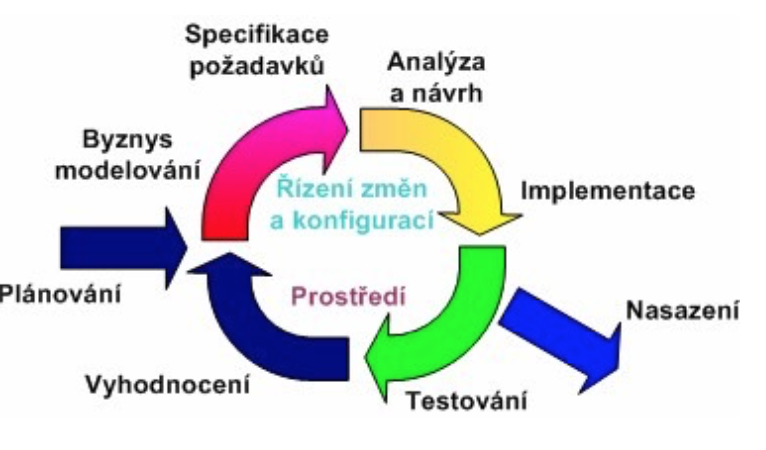
\includegraphics[width=9cm]{assets/swi2}}
